\section{Aufgabe 8}
\setcounter{section}{8}

In einer Studie zur Schlafdauer wurden folgende Schlafstunden pro Nacht von 40
Personen aufgezeichnet: (Es wird hier der Punkt zur Darstellung von Dezimal-
zahlen verwendet)

\begin{align*}
       8, 7, 6, 7.5, 9, 6.5, 7, 8.5, 6, 7&,\\
     7.5, 8, 5.5, 9, 7, 6.5, 7, 8, 9.5, 6&,\\
     7, 8.5, 6, 7.5, 8, 5.5, 7, 9, 6.5, 8&,\\
     7, 6, 8.5, 7.5, 9, 6.5, 8, 7, 9.5, 6&
\end{align*}

Konstruieren Sie ein Histogramm, um die Verteilung der Schlafdauer zu
visualisieren. Legen Sie die Intervalle so fest, dass sie die Verteilung der
Daten sinnvoll abbilden.

\begin{figure}[h]
    \centering
    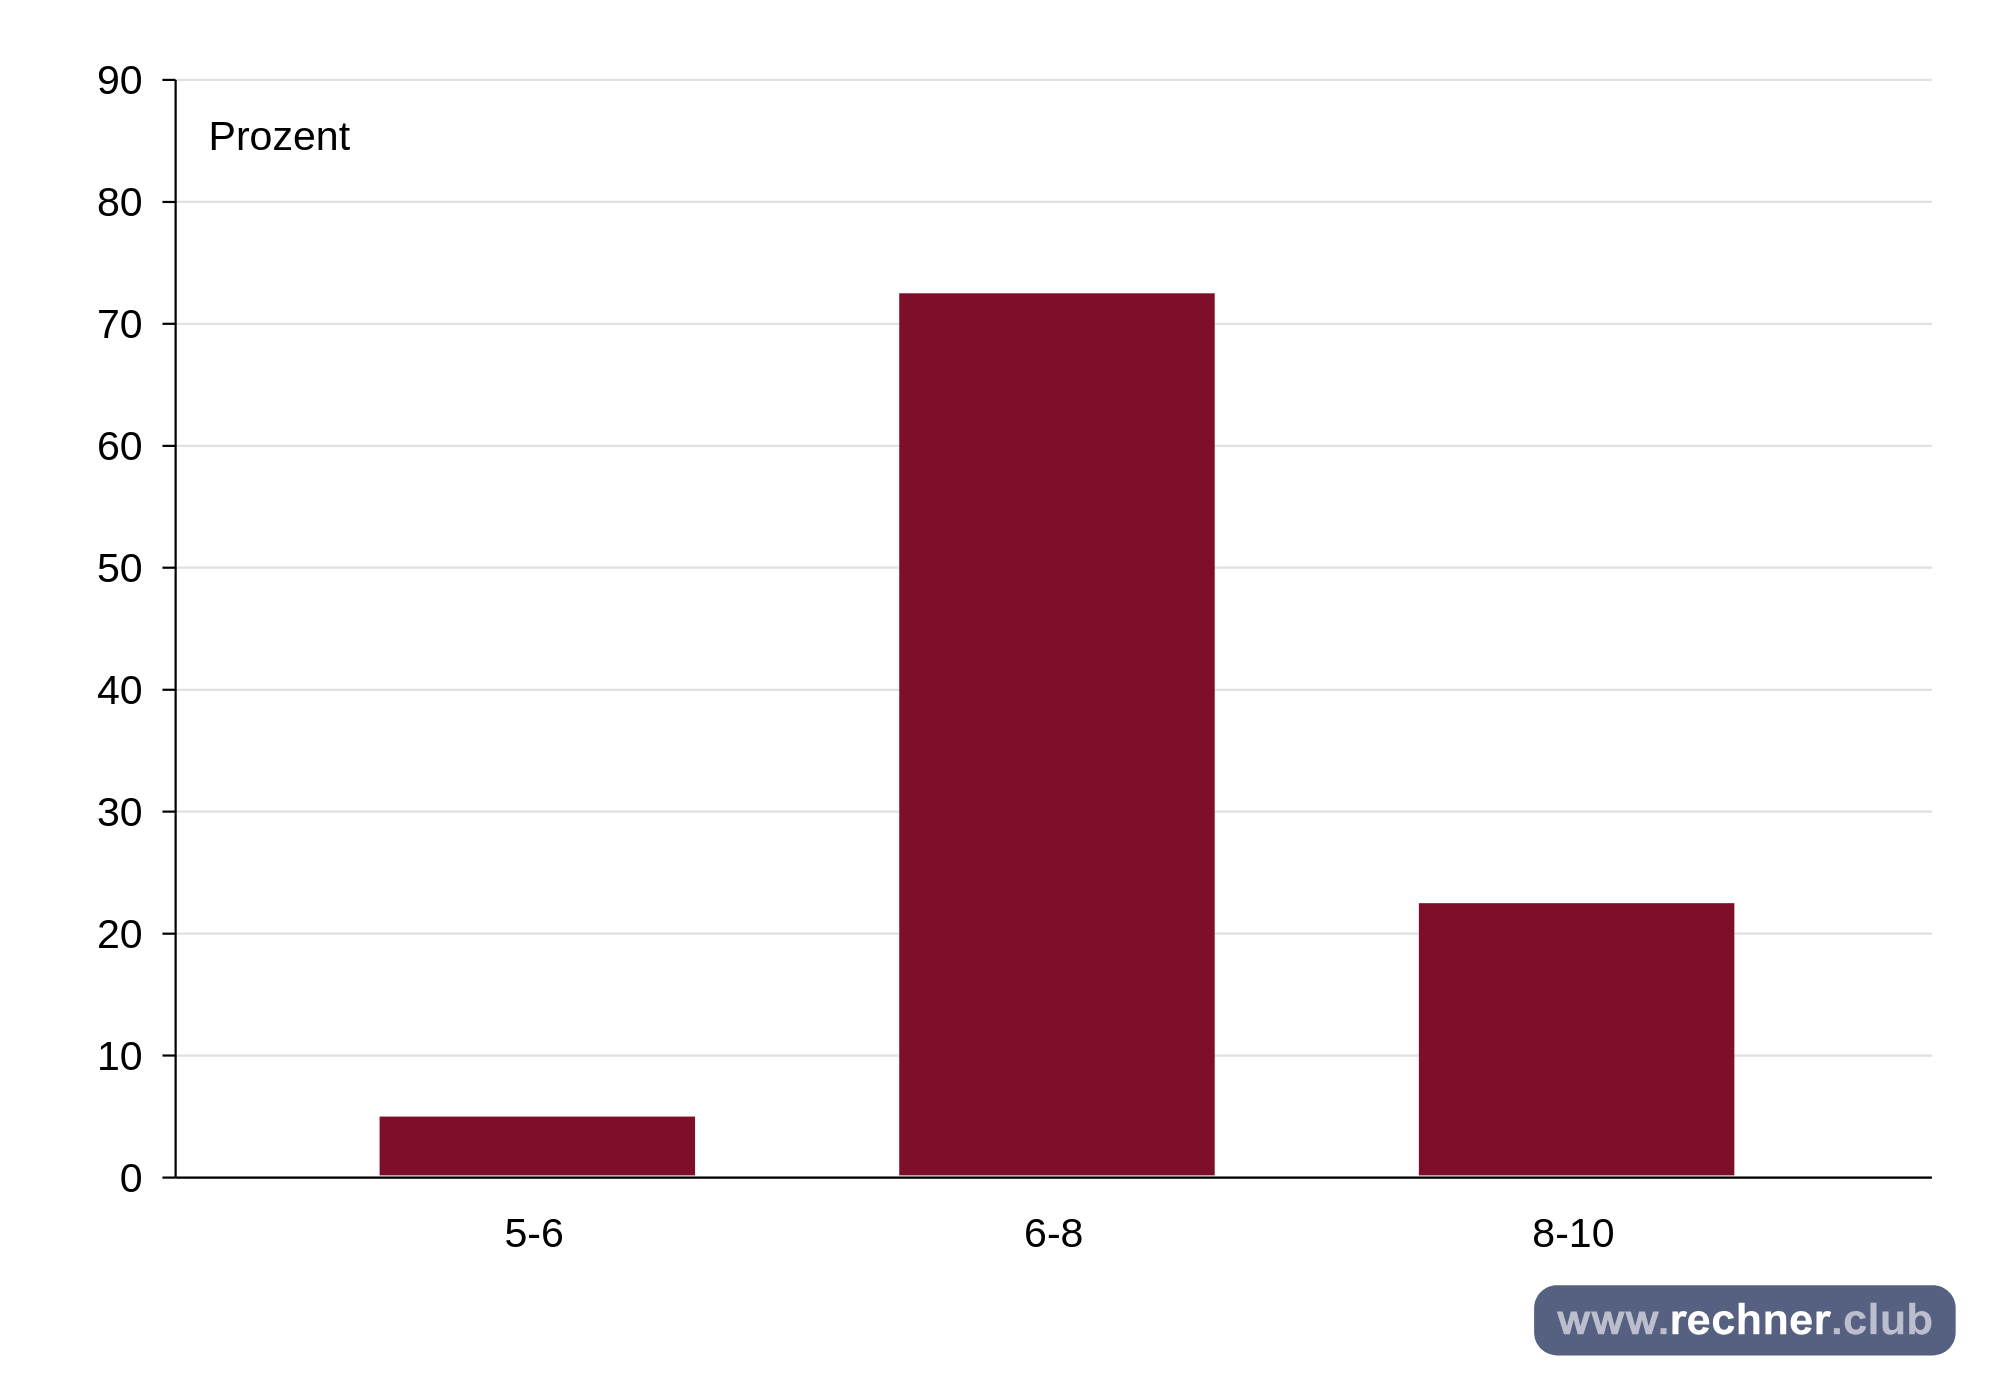
\includegraphics[width=0.8\textwidth]{./assets/abbildung-08-01.png}
    \caption{Verteilung der Schlafdauer}
\end{figure}
